\textbf{Summary.} The two distinct low-order intrinsic patterns we saw
when the $\pm$30/$\pm$45 rotator bins were added to the measured-intrinsic build
are \textbf{not a bug}. They are \textbf{two different observing epochs}
with different optical (thermal) state, and the rotator binning happens
to coincide exactly with that epoch split. Averaging the two epochs into
a single measured intrinsic is what inflated the residuals.

\subsection{The rotator/epoch confound}\label{the-rotatorepoch-confound}

Every $\pm$30/$\pm$45 visit was taken on a single night, \textbf{20260409}, 24
days after the March nights that carry the 0/$\pm$15/$\pm$60 rotators. So
``Family A'' vs ``Family B'' is really ``March'' vs ``April 9'':

{ % do not increment counter
\begin{longtable}[]{@{}llrl@{}}
\toprule\noalign{}
Night & rotator angles present & n visits & family \\
\midrule\noalign{}
\endhead
\bottomrule\noalign{}
\endlastfoot
20260315 & -60, -15, 0, 15, 60 & 61 & A \\
20260316 & -60, 0, 60 & 35 & A \\
20260317 & -60, -15, 0, 15, 60 & 72 & A \\
20260324 & -15 & 24 & A \\
\textbf{20260409} & \textbf{-45, -30, 30, 45} & \textbf{82} &
\textbf{B} \\
\end{longtable}
}

Family A (rot 0, $\pm$15, $\pm$60) = March 15--24, 192 visits. Family B (rot
$\pm$30, $\pm$45) = \textbf{entirely} April 9, 82 visits. A rotator-binned build
therefore mixes two epochs.

\subsection{What changed between the
epochs}\label{what-changed-between-the-epochs}

Per-visit median conditions, Family A (March) vs Family B (Apr 9):

{ % do not increment counter
\begin{longtable}[]{@{}
  >{\raggedright\arraybackslash}p{(\linewidth - 6\tabcolsep) * \real{0.2895}}
  >{\raggedleft\arraybackslash}p{(\linewidth - 6\tabcolsep) * \real{0.2895}}
  >{\raggedleft\arraybackslash}p{(\linewidth - 6\tabcolsep) * \real{0.2895}}
  >{\raggedleft\arraybackslash}p{(\linewidth - 6\tabcolsep) * \real{0.1316}}@{}}
\toprule\noalign{}
\begin{minipage}[b]{\linewidth}\raggedright
condition
\end{minipage} & \begin{minipage}[b]{\linewidth}\raggedleft
A (March)
\end{minipage} & \begin{minipage}[b]{\linewidth}\raggedleft
B (Apr 9)
\end{minipage} & \begin{minipage}[b]{\linewidth}\raggedleft
$\Delta$
\end{minipage} \\
\midrule\noalign{}
\endhead
\bottomrule\noalign{}
\endlastfoot
\textbf{z\_gradient} (M1M3 axial thermal) & \textbf{+0.09} &
\textbf{-0.30} & \textbf{-0.40} \\
cam / m2 / m1m3 air temp {[}$^\circ$C{]} & \textasciitilde12--13 &
\textasciitilde10--11.5 & -1.5 \\
outside\_temp {[}$^\circ$C{]} & 11.3 & 9.8 & -1.6 \\
dome\_delta\_t & -1.39 & -1.66 & -0.27 \\
cam\_m1m3\_delta\_t & -0.50 & -0.73 & -0.23 \\
azimuth & 270$^\circ$ & 314$^\circ$ & +44$^\circ$ \\
elevation & 69.8$^\circ$ & 69.9$^\circ$ & \textasciitilde0 (both in {[}65,75{]}) \\
\end{longtable}
}

The standout is \textbf{z\_gradient}: the M1M3 axial temperature
gradient \emph{flipped sign}, +0.09 $\to$ -0.30, on a \textasciitilde1.5 $^\circ$C
colder April-9 night. A change in the mirror's axial thermal gradient
directly drives low-order figure change (focus / astigmatism / spherical
print-through) --- a very plausible physical cause for two distinct
intrinsic patterns. (Azimuth also differs by \textasciitilde44$^\circ$, so
gravity-vector flexure is a secondary candidate, but elevation is
matched between the epochs, ruling out the dominant gravity term.)

\subsection{Evidence --- measured-intrinsic maps by rotator
angle}\label{evidence-measured-intrinsic-maps-by-rotator-angle}

These are the actual measured-intrinsic focal-plane maps, one per
rotator-angle bin, for Z5 and Z7. A \emph{stationary} intrinsic would
simply rotate coherently with the rotator across all 9 panels. Instead,
the March panels (blue, rot 0/$\pm$15/$\pm$60) form one coherent rotating
sequence, and the Apr-9 panels (red, rot $\pm$30/$\pm$45) break it --- a second
pattern.

\textbf{Z5 astigmatism:}
\pandocbounded{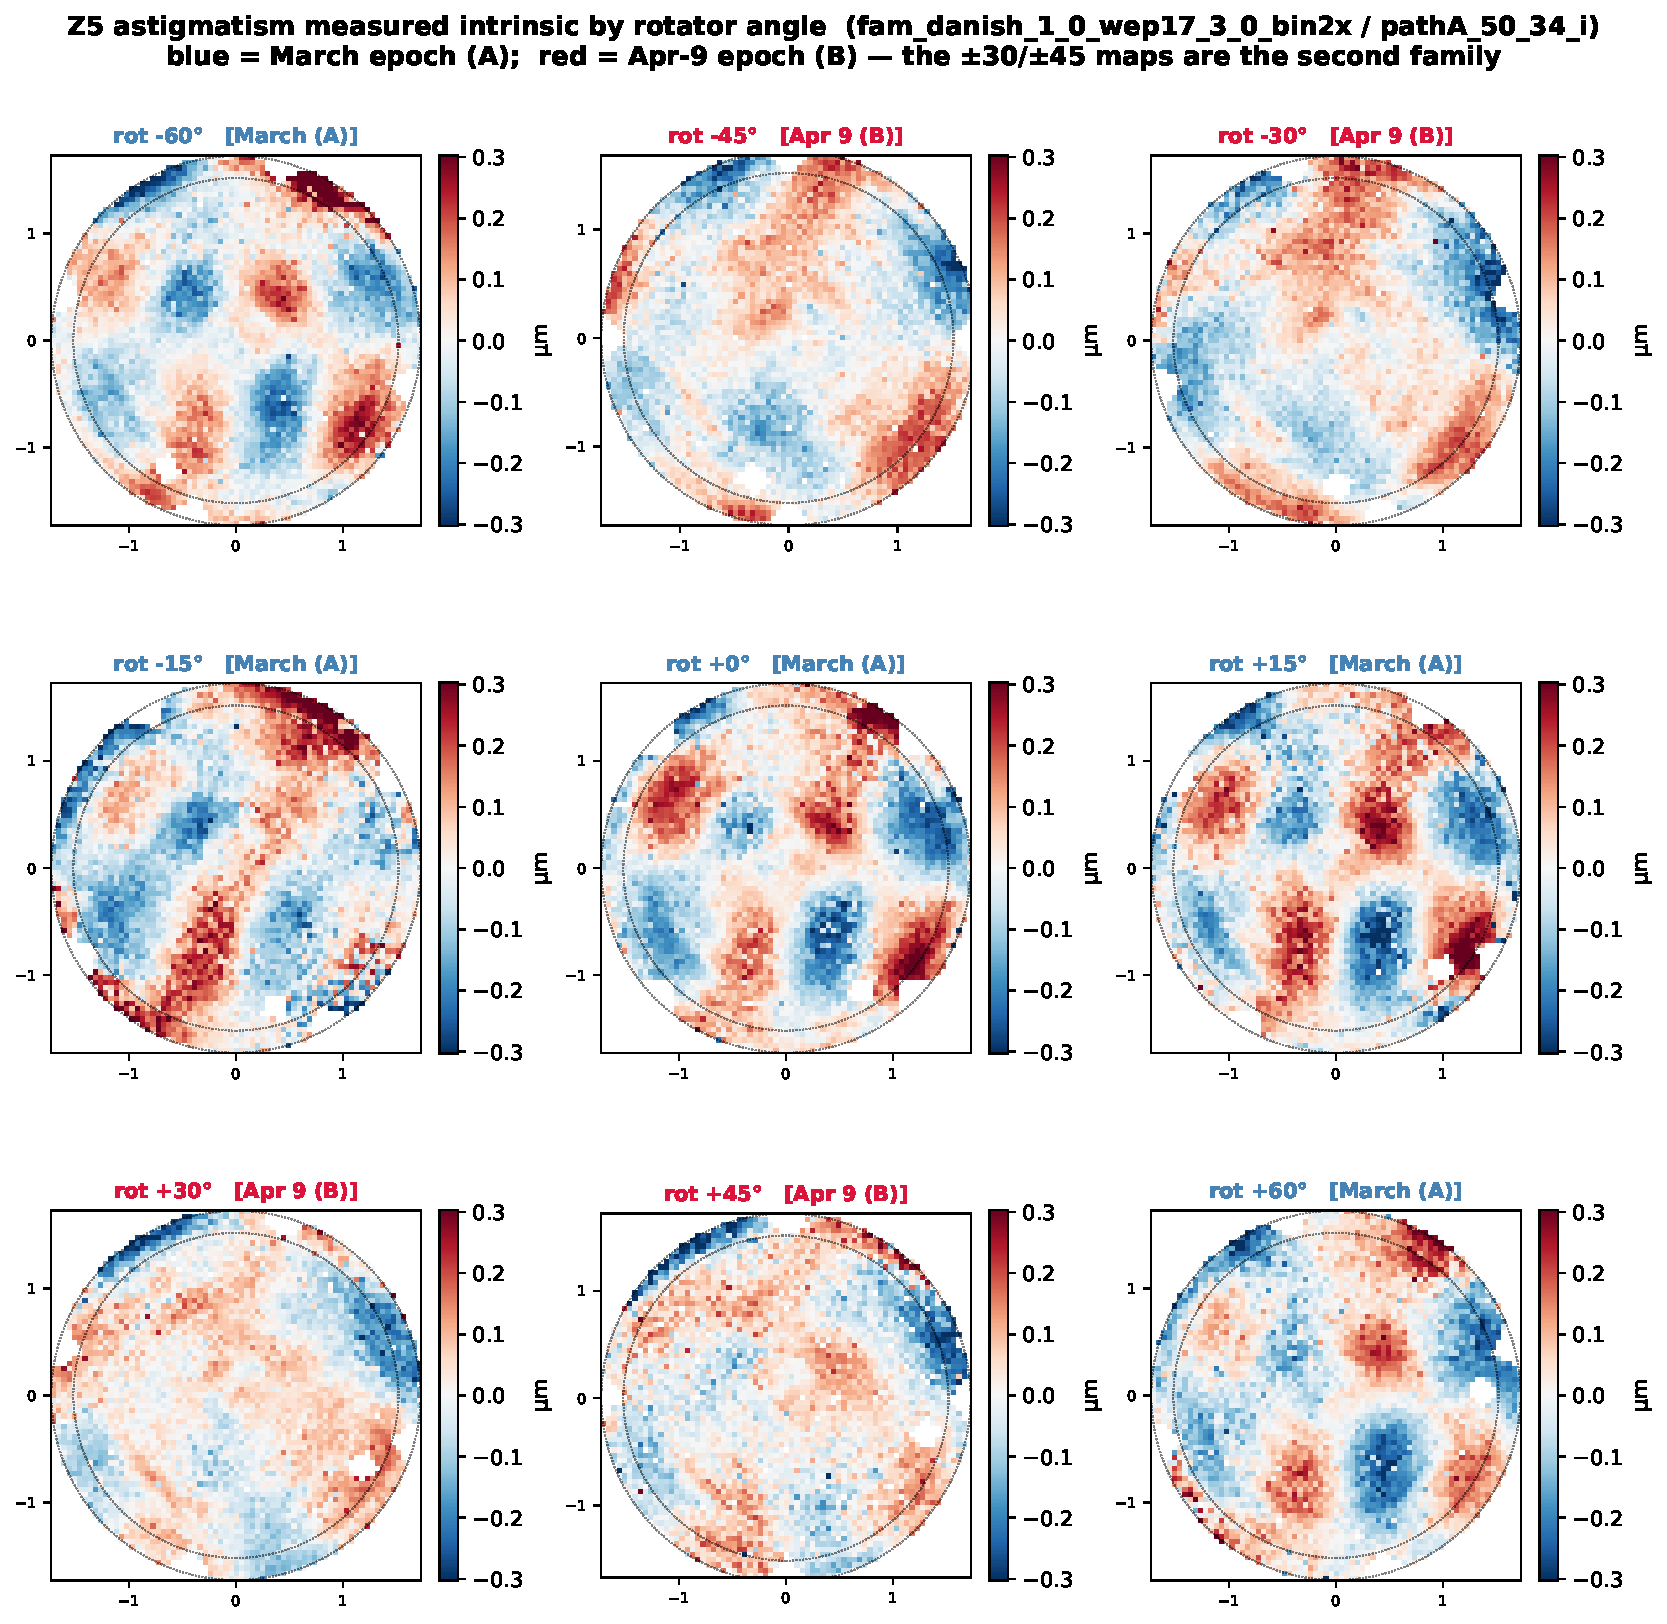
\includegraphics[keepaspectratio,alt={Z5 by rotator}]{figures/rotmaps_Z5_astigmatism}}

\textbf{Z7 coma:}
\pandocbounded{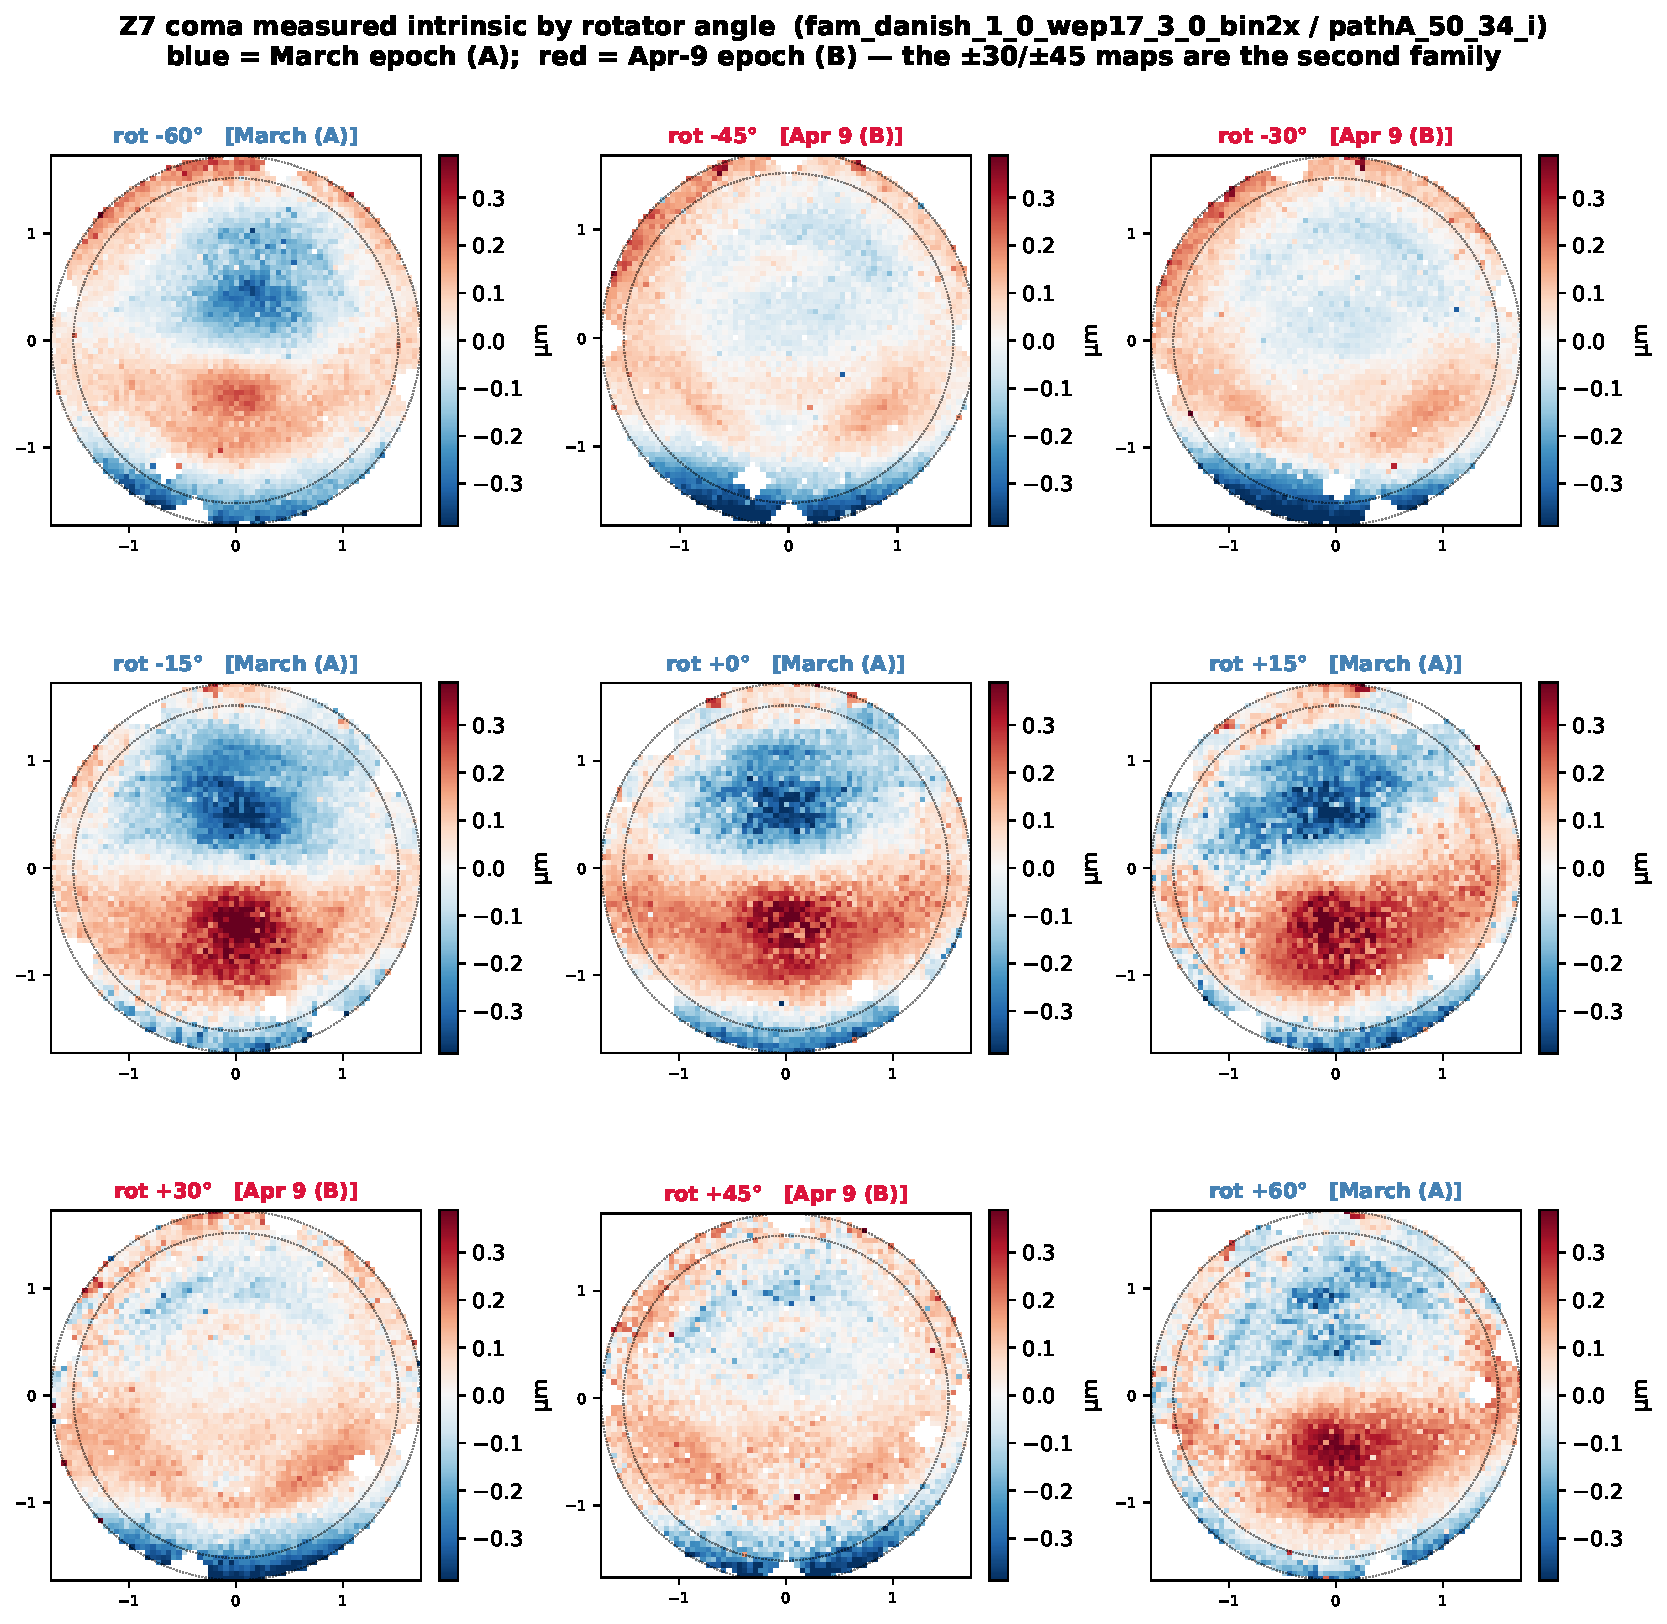
\includegraphics[keepaspectratio,alt={Z7 by rotator}]{figures/rotmaps_Z7_coma}}

\emph{Each panel is the measured intrinsic for that Zernike at one
rotator bin (\texttt{fam\_danish\_1\_0} / pathA\_50\_34, 73$\times$73 focal
grid; dotted rings = corner-WFS shell 1.518--1.725$^\circ$). Blue titles =
March epoch (A); red = April-9 epoch (B). The $\pm$30/$\pm$45 (red) maps do not
continue the March rotation sequence --- they are the second family.}

\subsubsection{The driver, and epoch-median
coefficients}\label{the-driver-and-epoch-median-coefficients}

\begin{figure}
\centering
\pandocbounded{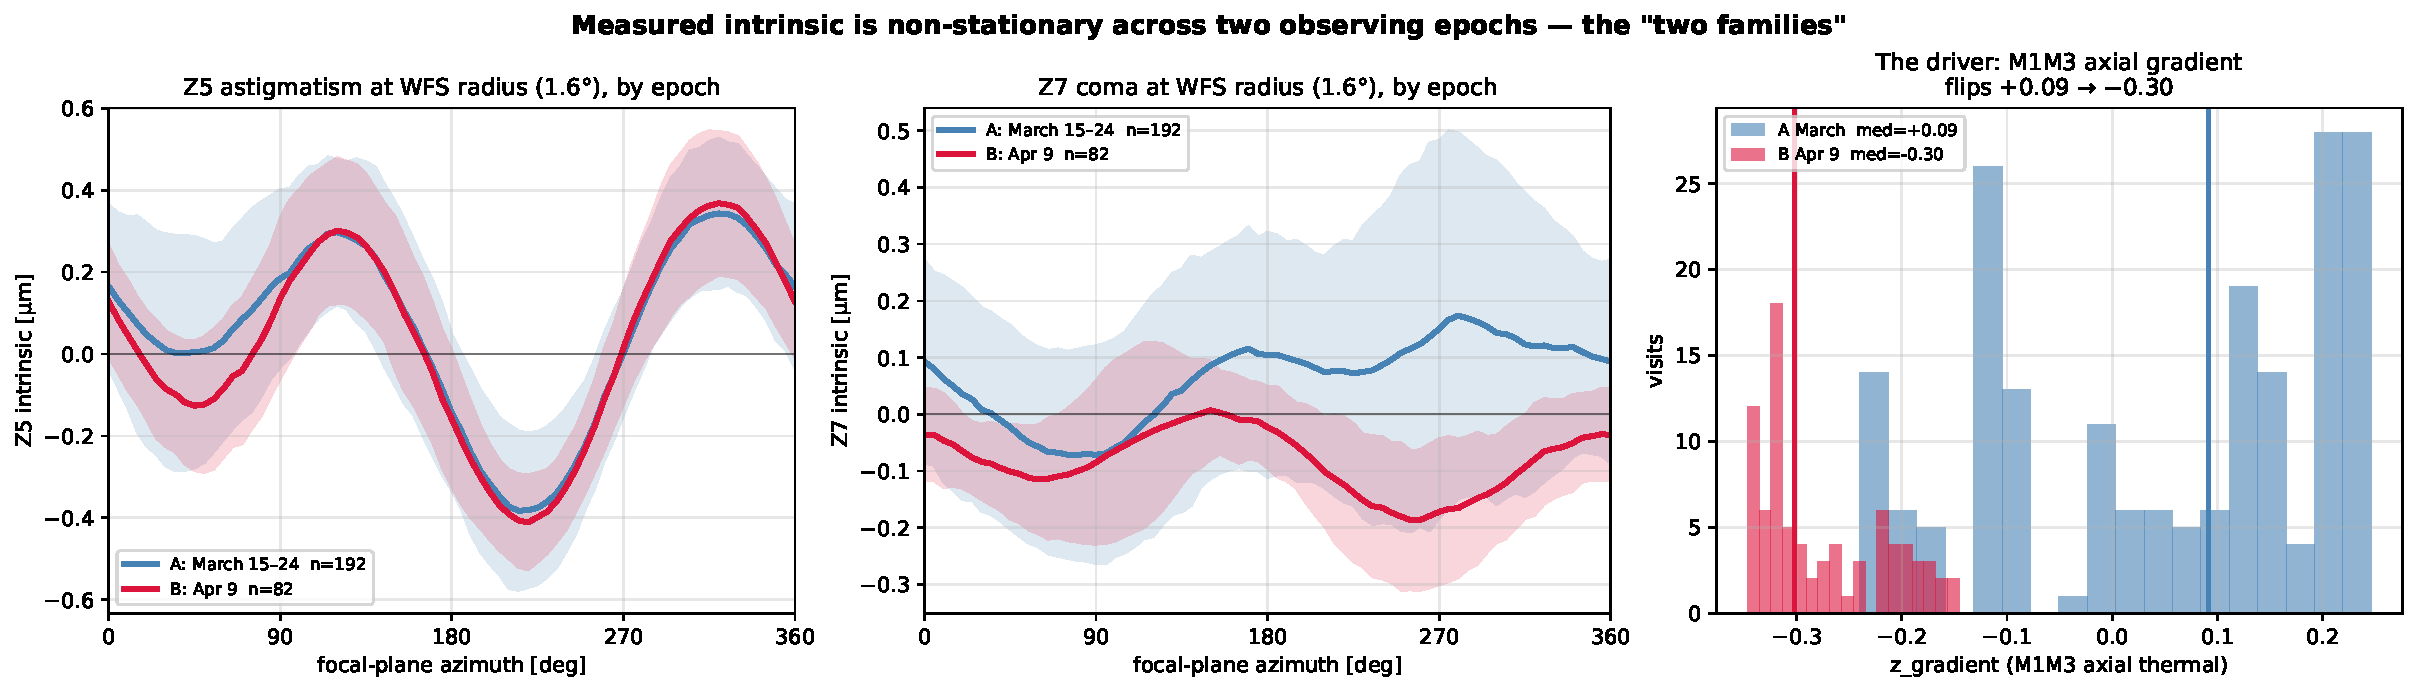
\includegraphics[keepaspectratio,alt={driver}]{figures/two_epochs_intrinsic}}
\caption{driver}
\end{figure}

\emph{Right panel: the M1M3 axial thermal gradient
(\texttt{z\_gradient}) cleanly separates the two epochs (+0.09 vs
-0.30).} Per-visit medians by epoch (raw DZ fit,
\texttt{fam\_danish\_1\_0}, wep 17.3.0):

{ % do not increment counter
\begin{longtable}[]{@{}lrrr@{}}
\toprule\noalign{}
term & A (March) & B (Apr 9) & $\Delta$ \\
\midrule\noalign{}
\endhead
\bottomrule\noalign{}
\endlastfoot
Z7 coma, field-mean & +0.060 & -0.108 & -0.168 \\
Z8 coma, field-mean & +0.117 & +0.006 & -0.111 \\
Z5 astig, c5 (field-varying) & -0.106 & -0.139 & -0.033 \\
\end{longtable}
}

\subsection{Conclusion}\label{conclusion}

This is real, not a build bug: \textbf{the measured intrinsic is not
stationary across the two epochs}, most clearly in low-order coma
(Z7/Z8) and traceable to the M1M3 axial thermal-gradient flip. Building
a single measured intrinsic over both epochs (which a rotator-binned
build does, because the $\pm$30/$\pm$45 bins are all April 9) averages two
different optical states and inflates the residuals. A build restricted
to the March epoch alone --- rotators \{0, $\pm$15, $\pm$60\} --- sees one
consistent state and gives smaller residuals.

\textbf{Implication:} epoch-restrict (or thermal-state-restrict) the
measured-intrinsic build, rather than pooling across nights with very
different M1M3 thermal gradients.
